\chapter{Toetsingsprocedures}
\label{ch:toetsingsprocedures}

In de voorbije hoofdstukken hebben we gezien hoe we aan de hand van steekproefonderzoek bepaalde kerngetallen over een populatie kunnen berekenen, bijvoorbeeld aan de hand van puntschatters of betrouwbaarheidsintervallen. We kunnen deze informatie ook gebruiken om bepaalde hypothesen over een populatie te toetsen. Een hypothese is een veronderstelling waarvan nog bewezen moet worden dat ze correct is. Het doel van een toetsingsprocedure is het testen van een hypothese omtrent de waarden van 1 of meerdere populatieparameters.

\begin{definition}[Statistische hypothese.]
  Een statistische hypothese\index{hypothese!statistische} is een uitspraak over de numerieke waarde van een populatieparameter.
\end{definition}

Voorbeelden van hypothesen:

\begin{itemize}
  \item Gemiddeld redt een superheld minstens 3,3 mensen per dag.
  \item De gemiddelde lengte van een superheld is minstens 120 cm.
  \item \dots
\end{itemize}

In dit hoofdstuk gaan we de algemene theorie over toetsen formuleren aan de hand van het testen van hypothesen over het populatiegemiddelde $\mu$, de $z$-toets. Naast de $z$-toets bestaan er echter nog vele andere statistische hypothesetoetsen die in specifieke situaties gebruikt kunnen worden. De meest geschikte statistische toets hangt o.a.~af van de populatiegrootheid in kwestie (gemiddelde, standaardafwijking, enz.), en veronderstellingen over de onderliggende stochastische verdeling van de populatie (normaal verdeeld of niet, enz,).

\section{Leerdoelen}
\label{sec:toetsingsprocedures-leerdoelen}

Na dit hoofdstuk moet je in staat zijn om:

\begin{itemize}
  \item De volgende begrippen uit dit hoofstuk uit te leggen:
  \begin{itemize}
    \item hypothesetoets, statistische hypothese, nulhypothese, alternatieve hypothese;
    \item teststatistiek, aanvaardings- en verwerpingsgebied, overschrijdingskans;
    \item $z$-toets, $t$-toets, linkszijdig, rechtszijdig, tweezijdige;
    \item Type I en Type II-fouten;
  \end{itemize}
  \item De algemene procedure voor een statistische toets te beschrijven;
  \item Uit de beschrijving van een situatie waarbij gevraagd wordt om een uitspraak over een populatiegemiddelde te verifiëren:
  \begin{itemize}
    \item te bepalen of er een $z$- of $t$-toets mag toegepast worden;
    \item uit de onderzoeksvraag af te leiden of de links-, rechts- of tweezijdige variant moet gebruikt worden;
  \end{itemize}
  \item Op een gegeven situatie correct de $z$- of $t$-toets toe te passen, d.w.z.:
  \begin{itemize}
    \item De nul- en alternatieve hypothese te formuleren (wiskundige notatie);
    \item De teststatistiek te berekenen;
    \item De kritieke grenswaarde(n) te berekenen en te bepalen of de teststatistiek in het aanvaardings- of verwerpingsgebied ligt;
    \item De overschrijdingskans te berekenen;
    \item Een correct besluit te kunnen trekken (nulhypothese verwerpen of niet);
    \item Een antwoord te formuleren op de onderzoeksvraag.
  \end{itemize}
\end{itemize}

\section{Elementen van een hypothesetoets}
\label{sec:elementen-hypothesetoets}

Algemeen gezien bestaat een toetsingsprocedure uit 4 elementen:
\begin{enumerate}
  \item \textbf{Nulhypothese}\index{nulhypothese}\index{hypothese!nul-} $H_{0}$: Deze hypothese proberen we te ontkrachten door een redenering in het ongerijmde. We gaan deze hypothese accepteren, tenzij de observaties uit de steekproef overtuigend wijzen op het tegendeel.
  \item \textbf{Alternatieve hypothese}\index{hypothese!alternatieve} $H_{1}$: Dit is meestal de hypothese die de onderzoeker wil bewijzen. Deze hypothese zal echter alleen worden geaccepteerd als de observaties uit de steekproef overtuigend wijzen op de juistheid ervan.
  \item \textbf{Teststatistiek}: De veranderlijke die berekend wordt uit de steekproef
  \item Aanvaardings- en kritiek gebied:
  \begin{itemize}
    \item  \textbf{Aanvaardingsgebied\index{aanvaardingsgebied}\index{gebied!aanvaardings-}}: Het gebied van waarden die de nulhypothese $H_{0}$ ondersteunt
    \item \textbf{Verwerpingsgbied\index{verwerpingsgebied}\index{gebied!verwerpings-}}: gebied dat waarden bevat die de nulhypothese verwerpen. Ook kritiek gebied\index{gebied!kritiek} genoemd.
  \end{itemize}
\end{enumerate}

Een alternatief voor de laatste stap is het berekenen van de \emph{overschrijdingskans} (zie verder).

De beslissing om de nulhypothese $H_{0}$ te verwerpen of te aanvaarden is gebaseerd op informatie uit een steekproef, getrokken uit de populatie waarover de hypothese is geformuleerd. De steekproefwaarden worden gebruikt om 1 enkele waarde van een teststatistiek te berekenen die de beslissing zal bepalen. Daartoe worden alle waarden die de teststatistiek kan aannemen, verdeeld in twee gebieden, enerzijds het aanvaardingsgebied en anderzijds het verwerpingsgebied. Indien de waarde van de teststatistiek ligt in het verwerpingsgebied, dan wordt de nulhypothese verworpen en de alternatieve hypothese aanvaard. Indien de waarde van de teststatistiek in het aanvaardingsgebied valt dan wordt de nulhypothese aanvaard.

\section{Toetsingsprocedure voor de \texorpdfstring{$z$}{z}-toets}
\label{sec:toetsingsprocedure-z-toets}

In de eerste toetsingsprocedure die we in deze cursus uitwerken, gaan we een uitspraak over het populatiegemiddelde $\mu$ verifiëren. Deze is algemeen bekend als de $z$-toets\index{$z$-toets}\index{toets!$z$-}.

\begin{enumerate}
  \item De vermoedens over de populatie worden vastgelegd in twee hypothesen $H_{0}$ en $H_{1}$. Voor de (rechtszijdige) $z$-toets is de nulhypothese dat het populatiegemiddelde $\mu$ een bepaalde waarde heeft, en de alternatieve hypothese dat $\mu$ \emph{groter} is.
  \item Het significantieniveau\index{significantieniveau}\index{niveau!significantie-} $\alpha$ en steekproefomvang $n$ worden vastgelegd. Je kan $\alpha$ in principe zelf kiezen (bv. 0,05)\footnote{Merk op dat het significantieniveau gerelateerd is aan het betrouwbaarheidsniveau $1-\alpha$. Zie Sectie~\ref{ssec:betrouwbaarheidsinterval-grote-steekproef}}. Hoe dichter het significantieniveau bij 0 ligt, hoe minder twijfel er is over het resultaat van de toets. Maar langs de andere kant wordt het ook moeilijker om de nulhypothese te verwerpen.
  \item De waarde van de toetsingsgrootheid in de steekproef wordt berekend. De uitkomst is bepalend voor de beslissing of we de nulhypothese $H_{0}$ kunnen verwerpen of niet. We weten dankzij de centrale limietstelling dat de kansverdeling van het steekproefgemiddelde $M \sim Nor( \mu, \frac{\sigma}{\sqrt{n}})$.
  \item Het kritieke gebied bepalen, of meer bepaald de grens tussen het aanvaardings- en het verwerpingsgebied. We zoeken een grenswaarde\index{kritieke grenswaarde} $g$ zodat:
  
  \begin{align}
  P(M > g) = \alpha & \Leftrightarrow P\left(Z> z=\frac{g-\mu}{\sigma/\sqrt{n}}\right) = \alpha & \mathrm{(normalisatie)}\\
  & \Leftrightarrow P\left(Z < z = \frac{g-\mu}{\sigma/\sqrt{n}}\right) = 1-\alpha & \mathrm{(100\%-regel)}
  \end{align}
  
  De $z$-waarde hangt af van het gekozen significantieniveau en kan worden opgezocht in een $z$-tabel of berekend worden met de R-functie \texttt{qnorm(1-alpha)}. Daaruit kunnen we dan $g$ afleiden:
  
  \begin{equation}
  z = \frac{g-\mu}{\sigma/\sqrt{n}} \Leftrightarrow g = \mu + z \frac{\sigma}{\sqrt{n}}
  \label{eq:kritieke-grenswaarde-z-toets}
  \end{equation}

  Alle waarden \emph{links} van $g$ vormen het aanvaardingsgebied. Waarden rechts, die dus ver van het $H_0$ veronderstelde populatiegemiddelde liggen, zijn het verwerpingsgebied. Zie ook Sectie~\ref{sec:kritieke-gebied}.
\end{enumerate}

\begin{example}
  \label{ex:hypothesetoets-dagelijkse-reddingen}
  Algemeen wordt aangenomen dat superhelden gemiddeld 3,3 mensen per dag redden. De onderzoekers krijgen echter gevoel dat dat niet zo is: ze hebben de indruk dat een superheld \emph{meer} dan $3,3$ mensen per dag redden.
  
  Ze gaan dit onderzoeken en voeren een steekproef uit bij $n = 30$ superhelden. In deze steekproef is het gemiddelde $\overline{x} = 3,483$ is. De standaardafwijking in de populatie is verondersteld gekend en is $\sigma = 0,55$.
  
  Kan hieruit besloten worden dat superhelden gemiddeld meer dan 3,3 mensen per dag redt?

  \begin{enumerate}
    \item We veronderstellen dat het aantal mensen dat een superheld redt normaal verdeeld  is en formuleren twee hypothesen omtrent de parameter $\mu$.
    \begin{itemize}
      \item $H_{0}$ = de nulhypothese (hetgeen we willen weerleggen). In dit geval \[ H_{0} : \mu = 3,3 \]
      \item $H_{1}$ = alternatieve hypothese (vermoeden dat we willen aantonen). In dit geval \[H_{1}= \mu > 3,3 \]
    \end{itemize}
  
    We veronderstellen in de redenering initieel dat de nulhypothese $H_{0}$ waar is. Indien het gemiddelde aantal mensen gered per dag $\overline{x}$ van de steekproef sterk afwijkt van de veronderstelde waarde, verwerpen we de nulhypothese $H_{0}$ en aanvaarden we de alternatieve hypothese $H_{1}$.
    
    Wat betekent nu ``sterk afwijken''? Zou je uit een populatie met gemiddelde van $3,3$ gemakkelijk een steekproef kunnen trekken met gemiddelde $3,483$? De centrale limietstelling (zie Sectie~\ref{sec:centrale-limietstelling}) laat ons toe de kans hiertoe te berekenen.
    
    \item Vastleggen significantieniveau $\alpha$ en steekproefomvang $n$. We willen een significantieniveau van 5\% kiezen, dus $\alpha = 0,05$. De steekproefomgang is gegeven en is hier $n = 30$.
    
    \item De waarde van de toetsingsgrootheid in de steekproef bepalen. We nemen hier het steekproefgemiddelde: $\overline{x} = 3,483$
    
    We veronderstellen in de redenering dat de nulhypothese $H_{0}$ waar is en dat we $\sigma$ goed kunnen schatten hebben ($\sigma = 0,55$). Dan geldt voor het steekproefgemiddelde $M$ volgens de centrale limietstelling dat:
    
    \[M \sim  Nor(\mu = 3,3; \sigma = \frac{0,55}{\sqrt{30}})\]
    
    De waarde $\overline{x} = 3,483$ bevindt zich erg rechts (zie Figuur~\ref{fig:hypothesetoets-reddingen-per-dag}). $\overline{x}$ ligt zelfs zo ver naar rechts dat de kans (indien $H_{0}$ waar is) om dergelijke geobserveerde waarde te krijgen of groter, zeer klein is. Een dergelijke geobserveerde waarde onder de nulhypothese kan dus moeilijk verklaard worden door louter toeval. Intu\"itief voelen we dus aan dat hoe verder de geobserveerde waarde $\overline{x}$ zich bevindt in de rechtse richting, hoe meer we geneigd zijn om de nulhypothese te verwerpen. Maar wat is te ver en wat niet?
    
    \item De kritieke grenswaarde berekenen. De $z$-waarde voor een significantieniveau van $0,05$ is 1,645\footnote{In R kan je dit berekenen met \texttt{qnorm(1 - 0.05)}}.
    
    \[ g = \mu + z \times \frac{\sigma}{\sqrt{n}} = 3,3 + 1,645 \times \frac{0,55}{\sqrt{30}} \approx 3,45 \]
    
    Het steekproefgemiddelde $\overline{x} = 3,483$ ligt nog verder van $\mu = 3,3$ dan de grenswaarde $g = 3,45$. De kans is heel klein dat zo'n steekproef getrokken wordt uit een populatie met dit gemiddelde. Slechts in 34 steekproeven op 1000 zal een dergelijke gebeurtenis optreden. Met andere woorden, de steekproefwaarde ligt in het verwerpingsgebied. We kunnen dus $H_0$ verwerpen en besluiten dat superhelden inderdaad \emph{meer} dan 3,3 mensen per dag redden.
  \end{enumerate}

\end{example}

\begin{exercise}
  Kunnen we in Voorbeeld~\ref{ex:hypothesetoets-dagelijkse-reddingen} zomaar veronderstellen dat het gemiddelde normaal verdeeld is? Waarom (niet)?
\end{exercise}

\begin{figure}
  \centering
  \begin{tikzpicture}
    \begin{axis}[
        domain=3:3.6, samples=100,
        axis lines*=left, xlabel=$x$,
        every axis y label/.style={at=(current axis.above origin),anchor=south},
        every axis x label/.style={at=(current axis.right of origin),anchor=west},
        height=5cm, width=12cm,
        xtick={3.3,3.483}, ytick=\empty,
        xticklabels={$\mu$,$\overline{x}$},
        enlargelimits=false, clip=false, axis on top,
        grid = minor
      ]
      \addplot [fill=cyan!20, draw=none, domain=3:3.465] {gauss(3.3,0.1004)} \closedcycle;
      \addplot [fill=none, draw=black, domain=3:3.6] {gauss(3.3,0.1004)} \closedcycle;
      \draw [-](axis cs:3.465,1.6) -- (axis cs:3.465,0);
      \node at (axis cs:3.465,1.8) {3.465};
      \node at (axis cs:3.483,-0.7) {3.483};
      \node at (axis cs:3.3,-0.7) {3.3};
    \end{axis}
  \end{tikzpicture}
  \caption{Verdeling van het aantal mensen dat gemiddeld per dag gered wordt door een superheld (Voorbeeld~\ref{ex:hypothesetoets-dagelijkse-reddingen}). De kansverdeling voor het steekproefgemiddelde is normaal verdeeld met $\mu = 3,3$ en $\sigma = 0,55$. Het steekproefgemiddelde $\overline{x} =3,483$. De grens voor aanvaarding/verwerping van $H_{0}$ is 3.465.}
  \label{fig:hypothesetoets-reddingen-per-dag}
\end{figure}

\section{Kritieke gebied}
\label{sec:kritieke-gebied}

De formule voor de berekening van de grenswaarde (zie Formule~\ref{eq:kritieke-grenswaarde-z-toets}) is gebaseerd op de centrale limietstelling, en meer bepaald betrouwbaarheidsintervallen.

De kritieke grenswaarde vormt een betrouwbaarheidsinterval rond $\mu$ met een gekozen zekerheidsniveau. Als we bijvoorbeeld stellen dat $\alpha = 0.05$, weten we vanuit de centrale limietstelling dat we kunnen verwachten dat als we herhaaldelijk voldoende steekproeven uit deze populatie nemen, in 95\% van de gevallen het steekproefgemiddelde binnen dit betrouwbaarheidsgeval zal liggen.

Als we de redenering omkeren, en een steekproef genomen hebben waar het gemiddelde $\overline{x}$ \emph{niet} binnen dit betrouwbaarheidsinterval ligt, dan is de kans heel klein (kleiner dan 5\%) dat deze uit een populatie getrokken is met het veronderstelde gemiddelde $\mu$. In dat geval kunnen we de nulhypothese dus verwerpen.

In Voorbeeld~\ref{ex:hypothesetoets-dagelijkse-reddingen} is de kritieke grenswaarde het getal $g$ waarvoor geldt dat

\[ P(M > g) = \alpha \]

wat dan wordt verder uitgewerkt als:

\[ P(Z > \frac{g - \mu}{\frac{\sigma}{\sqrt{n}}}) = \alpha \]

waaruit volgt dat:

\begin{equation}
  \label{eq:kritieke-waarde-rechtszijdig}
  g = \mu + z \times \frac{\sigma}{\sqrt{n}}
\end{equation}

\section{Overschrijdingskans}
\label{sec:overschrijdingskans}

Een karakteristiek die gebruikt wordt om weer te geven hoe sterk de geobserveerde waarde afwijkt van $H_{0}$, is de overschrijdingskans (probability value of ook $p$-waarde\index{$p$-waarde}). Dit vormt een alternatieve manier om te bepalen of de nulhypothese al dan niet verworpen kan worden.

\begin{definition}[overschrijdingskans]
  De \emph{overschrijdingskans}\index{overschrijdingskans} is de kans, indien de nulhypothese waar is, om een waarde te verkrijgen van de toetsingsgrootheid die minstens even extreem is als de geobserveerde waarde.
\end{definition}

\begin{definition}[statistische significantie]
  In een statistische hypothesetoets heeft men een \emph{statistisch significant}\index{significant} resultaat behaald wanneer de geobserveerde overschrijdingskans $p$ van de teststatistiek lager is dan het significantieniveau $\alpha$. De $p$-waarde wordt onder het gekozen significantieniveau beschouwd als te extreem om de veronderstelling dat de nulhypothese waar is aan te houden.
\end{definition}

\begin{example}
  In het onderzoek naar het aantal dagelijkse reddingen door superhelden (Voorbeeld~\ref{ex:hypothesetoets-dagelijkse-reddingen}) kan de overschrijdingskans als volgt berekend worden:
  
\[ P(M > 3,483) = P \left(Z> \frac{3,483 - 3,3}{\frac{\sigma}{\sqrt{n}}}\right) = P (Z > 1,822) = 0,0344 \]
\end{example}

Als de overschrijdingskans of $p$-waarde kleiner is dan de onbetrouwbaarheidsdrempel dan moet $H_{0}$ verworpen worden, is de $p$-waarde gelijk of groter dan $\alpha$ dan mag je $H_{0}$ niet verwerpen. In ons geval is de $p$-waarde $0,0344$ en die is kleiner dan $\alpha = 0,05$ dus moeten we $H_{0}$ verwerpen.

\begin{itemize}
  \item $p$-waarde $< \alpha \Rightarrow$ $H_{0}$, verwerpen want de gevonden waarde voor $\overline{x}$ is te extreem;
  \item $p$-waarde $\geq \alpha \Rightarrow$ $H_{0}$ niet verwerpen, want de gevonden waarde voor $\overline{x}$ kan nog verklaard worden door toeval.
\end{itemize}

\section{Eenzijdig of tweezijdig toetsen}
\label{sec:eenzijdig-of-tweezijdig}

In Voorbeeld~\ref{ex:hypothesetoets-dagelijkse-reddingen} gaat het om een hypothese waar we vermoeden dat het populatiegemiddelde \emph{hoger} ligt dan een bepaalde waarde. We twijfelen dus aan de nulhypothese als ons steekproefgemiddelde significant boven het vooropgestelde gemiddelde $\mu = 3,3; \alpha = 0,05$ ligt. Het kritieke gebied om $H_{0}$ te verwerpen ligt dus aan de rechterzijde van de curve en we noemen deze toets dan ook rechtszijdig.

We zouden ook een toets kunnen maken waar we denken dat de superhelden gemiddeld \emph{minder} mensen redden per dag. Dan ligt het kritieke gebied aan de linkerzijde en noemen we de toets linkszijdig.

\begin{exercise}
  \label{ex:kritieke-waarde-linkszijdig}
  Wat zou je in vergelijking \ref{eq:kritieke-waarde-rechtszijdig} moeten veranderen opdat je de correcte kritieke waarde zou berekenen voor een linkszijdige $z$-toets?
\end{exercise}

Soms kan het ook zijn dat er tweezijdig moet getoetst worden. De alternatieve hypothese wordt dan geformuleerd als zijnde dat het populatiegemiddelde verschillend is van de opgegeven waarde. Er moeten dan twee kritieke grenswaarden berekend worden namelijk de linker- en de rechter grenswaarden.

\begin{equation}
  g = \mu \pm z \times \frac{\sigma}{\sqrt{n}}
  \label{eq:kritieke-waarde-tweezijdig}
\end{equation}

De totale oppervlakte van het kritieke gebied moet $\alpha$ zijn, en je moet er rekening mee houden dat zowel links als rechts een gebied met telkens oppervlakte $\alpha / 2$ samen het kritieke gebied vormen. Je moet dan ook de overeenkomstige $z$-waarde kiezen. Als we opnieuw significantieniveau $\alpha = 0,05$ nemen, zoeken we dus de $z$ waarde waarvoor geldt dat;

\[P(Z < -z) + P(Z > z) = \alpha \Leftrightarrow 2 P(Z>z) = \alpha \Leftrightarrow P(Z < z) = 1-\frac{\alpha}{2} = 0,975\]

De overeenkomstige $z$-waarde is dan ongeveer 1.96 (op te zoeken in de $z$-tabel of in R met \texttt{qnorm(.975)}).

De drie vormen van de $z$-toets worden samengevat in tabel~\ref{tab:toetsingsprocedures}.

\begin{table}
  \centering
  \begin{tabular}{l|ccc}
    \toprule
    Doel              & \multicolumn{3}{l}{\parbox{.5\textwidth}{Test op gemiddelde waarde $\mu$ van de populatie aan de hand van een steekproef van $n$ onafhankelijke steekproefwaarden}} \\
    \midrule
    Voorwaarde        & \multicolumn{3}{l}{\parbox{.5\textwidth}{De populatie is willekeurig verdeeld, $n$ voldoende groot}} \\
    \midrule
    Type test         & Tweezijdig           & Eenzijdig links & Eenzijdig rechts \\
    \midrule
    $H_{0}$           & $\mu = \mu_{0}$      & $\mu = \mu_{0}$ & $\mu = \mu_{0}$  \\
    $H_{1}$           & $\mu \neq \mu_{0}$   & $\mu < \mu_{0}$ & $\mu > \mu_{0}$  \\
    Verwerpingsgebied & $\left|z\right| > g$ & $z< -g $        & $z>g$            \\
    Teststatistiek    & \multicolumn{3}{c}{$z = \frac{\overline{x} - \mu_{0}}{\frac{\sigma}{\sqrt{n}}}$} \\
    \bottomrule
  \end{tabular}
  \caption{Samenvatting verschillende vormen van de $z$-toets}
  \label{tab:toetsingsprocedures}
\end{table}

\section{De \texorpdfstring{$z$}{z}-toets in R}
\label{sec:z-toets-R}

Het codevoorbeeld hieronder is de uitwerking van Voorbeeld~\ref{ex:hypothesetoets-dagelijkse-reddingen} in R.

\lstinputlisting{data/z-toets.R}

\begin{figure}
  \centering
  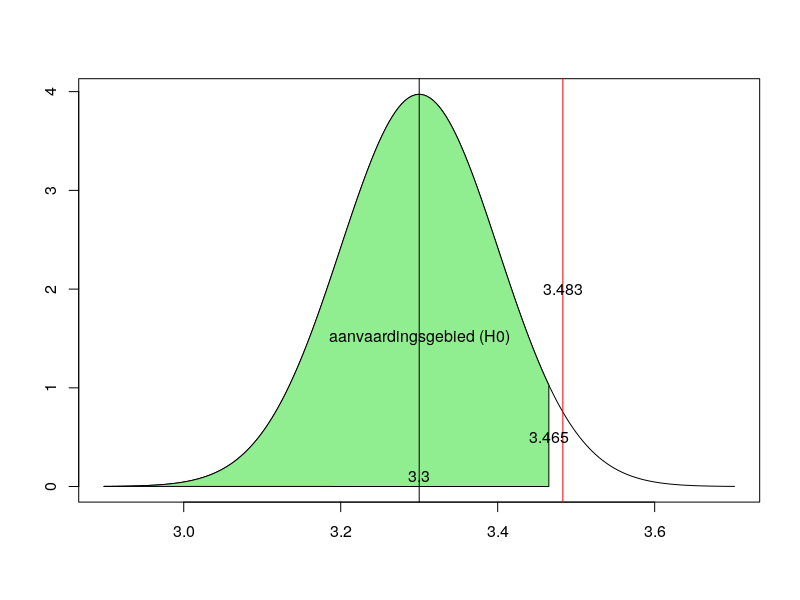
\includegraphics[width=\textwidth]{z-toets-reddingen}
  \caption{Plot in R van de situatie van Voorbeeld~\ref{ex:hypothesetoets-dagelijkse-reddingen}}
\end{figure}

\section{Voorbeelden}
\label{sec:toetsingsprocedures-voorbeelden}

\begin{example}
  Bij een aselecte steekproef van 50 waarnemingen vinden we volgende grootheden:
  \begin{itemize}
    \item $\overline{x} = 25$
    \item $s = \sqrt{55} = 7,41$
  \end{itemize}
  
  We willen weten of er reden is om aan te nemen dat $\mu$ van de populatie kleiner is dan 27.
  
  \begin{enumerate}
    \item Bepalen van de hypothesen: 
    
    $H_{0} : \mu = 27$ en $H_{1}: \mu < 27$.
    
    \item Vastleggen significantieniveau $\alpha$ en steekproefomvang $n$:
    
    $\alpha = 0,05$ en $n=50$.
    
    \item Waarde toetsingsgrootheid bepalen. 
    
    We kiezen hiervoor het steekproefgemiddelde $M$. Volgens de centrale limietstelling geldt:
    
    \[ M \sim Nor(\mu = 27, \frac{\sigma}{\sqrt{n}}) \]
    De toetsingsgrootheid is
    \[ Z = \frac{\overline{x} - \mu}{\frac{\sigma}{\sqrt{n}}} = \frac{25-27}{\sqrt\frac{55}{50}} \approx -1,91\]
    
    \item Overschrijdingskans berekenen.
    
    We vinden een overschrijdingskans van het gemiddelde van \texttt{pnorm(-1.91)} of ongeveer $0,0281$. Bij een significantieniveau van 0,05 duidt dit er op dat we $H_{0}$ mogen verwerpen.
    
    \item Bereken en teken kritiek gebied.
    
    \[ g = \mu - z \times \frac{\sigma}{\sqrt{n}} \]
    en dus
    
    \[ g = 27 - 1,645 \times \sqrt{\frac{55}{50}} \]
    \[ g =  25,27470944 \]
    
    We vinden dus dat $\overline{x} < g$ komen tot hetzelfde besluit, nl.~dat we $H_{0}$ kunnen verwerpen.
    
  \end{enumerate}
\end{example}

\begin{example}
  In een onderzoek naar het kleingeld dat in de zakken van van onze superhelden zit, stellen de onderzoekers dat zij gemiddeld 25 euro op zak hebben. Ze gaan ervan uit de spreiding $\sigma = 7$ is. Verder zijn de gegevens van de aselecte steekproef van omvang $n=64$ beschikbaar met gemiddeld zakgeld $\overline{x}$ van 23 euro. Voor het significantieniveau kiezen ze $\alpha = 0,05$.
  
  \begin{enumerate}
    \item Bepalen van de hypothesen.
    
    $H_{0} : \mu = 25$ en $H_{1}: \mu \neq 25$.
    
    \item Vastleggen significantieniveau $\alpha$ en steekproefomvang $n$.
    
    $\alpha = 0,05$ en $n=64$.
    
    \item Bepalen van de kritieke grenzen.
    
    \[ g_{1} = \mu - z \times \frac{\sigma}{\sqrt{n}} = 23,28 \]
    
    \[ g_{2} = \mu + z \times \frac{\sigma}{\sqrt{n}} = 26,72 \]
    
    \item Kritiek gebied.
    
    We vinden dat $\overline{x}$ in het kritieke gebied ligt (want $\overline{x} = 23 < g_1 = 23,28$), dus mogen we $H_{0}$ verwerpen.
    
  \end{enumerate}
\end{example}

\section{De \texorpdfstring{$t$}{t}-toets}
\label{sec:t-toets}

Bij de $z$-toets gaan we uit van een aantal veronderstellingen waar we rekening moeten mee houden:

\begin{itemize}
  \item De steekproef moet voldoende groot zijn ($n \ge 30$);
  \item De variatie van de toetsingsgrootheid moet normaal verdeeld zijn;
  \item We veronderstellen dat de standaardafwijking van de populatie, $\sigma$, gekend is.
\end{itemize}

De eerste drie voorwaarden maken dat de centrale limietstelling kan toegepast worden.

Soms zijn deze veronderstellingen niet geldig en mogen we dan ook de $z$-toets \emph{niet} gebruiken! In deze gevallen kunnen we wel gebruik maken van de Student-$t$ verdeling. In de $t$-toets\index{$t$-toets}\index{toets!$t$-} wordt er wel van uit gegaan dat de onderzochte variabele normaal verdeeld is.

De Student-$t$ verdeling dankt zijn naam aan statisticus William Sealy Gosset\index{Gosset, William Sealy}. Hij werkte in de Guinness-brouwerij en gebruikte statistische methoden om de kwaliteit van het bier te garanderen. Zijn werkgever beschouwde dit als een bedrijfsgeheim en stond Gosset niet toe om te publiceren onder zijn eigen naam. Daarom gebruikte hij het pseudoniem Student\index{Student}.

De formule voor de kritieke grenswaarde bij de $t$-toets aangepast naar:

\begin{equation}
g = \mu \pm t \times \frac{s}{\sqrt{n}}
\label{eq:kritieke-waarde-t-toets}
\end{equation}

Voor het bepalen van de $t$-waarde hebben we het aantal vrijheidsgraden nodig, $n-1$. Om de standaardafwijking te schatten, gebruiken we de steekproefstandaardafwijking, $s$.

\begin{example}
  \label{ex:t-toets-dagelijkse-reddingen}
  Stel dat de onderzoekers van de superhelden uit Voorbeeld~\ref{ex:hypothesetoets-dagelijkse-reddingen} door tijdsdruk niet in staat waren om een voldoende grote steekproef te nemen en slechts $n = 25$ observaties gedaan hebben, met hetzelfde steekproefgemiddelde $\overline{x} = 3,483$. De standaardafwijking in deze steekproef bleek $s = 0,55$.
  
  Kunnen we in deze omstandigheden, met eenzelfde significantieniveau $\alpha = 0,05$, het besluit dat superhelden dagelijks \emph{meer} dan 3,3 mensen redden aanhouden?
  
  \begin{enumerate}
    \item Bepalen van de hypothesen.
    
      $H_{0} : \mu = 3,3$ en $H_{1}: \mu > 3,3$.
    
    \item Vastleggen significantieniveau $\alpha$ en steekproefomvang $n$.
    
    $\alpha = 0,05$ en $n=25$.
    
    \item Bepalen van de kritieke grenswaarde.
    
    \[ g_{2} = \mu + t \times \frac{s}{\sqrt{n}} \approx 3,3 + 1,711 \times \frac{0,55}{\sqrt{25}} \approx 3.488 \]
    
    De waarde voor $t$ wordt in R berekend met \texttt{qt(1-a, df = n - 1)} (met \texttt{a} het significantieniveau en \texttt{df} het aantal vrijheidsgraden.)
    
    \item Conclusie.
    
    We vinden dat $\overline{x} = 3,483$ kleiner is dan de kritieke grenswaarde en dus in het aanvaardingsgebied ligt. Met andere woorden, we mogen $H_{0}$ \emph{niet} verwerpen.
  \end{enumerate}

  Met andere woorden, ook al krijgen we gelijkaardige resultaten in onze steekproef, kunnen we niet hetzelfde besluit trekken. Omdat onze steekproef te klein is, is er grotere onzekerheid of de waarde van het steekproefgemiddelde extreem genoeg is om de nulhypothese te verwerpen.
  
  Hieronder vind je de uitwerking van dit voorbeeld in R.
\end{example}

\lstinputlisting{data/t-toets.R}

\begin{figure}
  \centering
  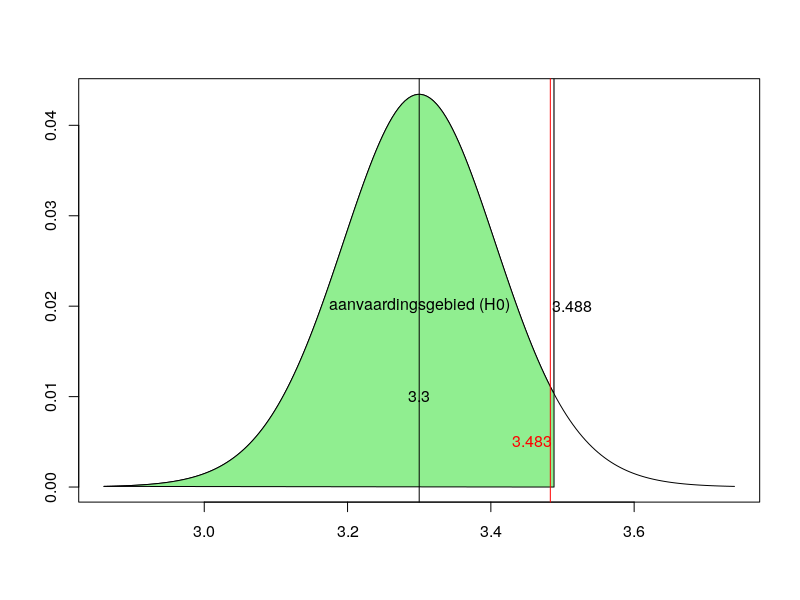
\includegraphics[width=\textwidth]{t-toets-reddingen}
  \caption{Plot in R van de situatie van Voorbeeld~\ref{ex:t-toets-dagelijkse-reddingen}}
\end{figure}

\begin{example}
  Een uitbraak van een door Salmonella veroorzaakte ziekte werd toegeschreven aan vanille-ijs van een bepaalde fabriek~\autocite{Lindquist}. Wetenschappers hebben het niveau van Salmonella gemeten in 9 willekeurig genomen steekproeven.
  
  De niveaus (in MPN/g\footnote{Most Probable Number. Zie bv.~\url{http://www.microbiologie.info/mpn-methode.html} voor meer uitleg over deze methode.}) zijn de volgende:
  
    \begin{center}
    \begin{tabular}{|l|l|l|l|l|}
      \hline
      0,593 & 0,142 & 0,329 & 0,691 & 0,231 \\ \hline
      0,793 & 0,519 & 0,392 & 0,418 &       \\ \hline
    \end{tabular}
  \end{center}

  Is er reden om aan te nemen dat het Salmonella-niveau in het ijs significant groter is dan 0,3 MPN/g? We zullen gebruik maken van de R-functie \texttt{t.test} om deze vraag te beantwoorden. Lees zelf de help-pagina van deze functie om de mogelijke opties te leren kennen.
  
  \begin{enumerate}
    \item Bepalen van de hypothesen
    
    $H_0: \mu = 0.3, H_1: \mu > 0,3$
    
    \item Vastleggen significantieniveau $\alpha = 0.05$ (in R moet je het betrouwbaarheidsniveau $1-\alpha$ opgeven, dus 0,95) en steekproefomvang $n = 9$
    
    \item Bepalen overschrijdingskans. Het gaat hier over een rechtszijdige toets, wat aangegeven wordt met de optie \texttt{alternative="greater"}. Het gekozen betrouwbaarheidsniveau is de standaardwaarde voor deze functie en moet niet expliciet meegegeven worden.
    
\begin{lstlisting}
x <- c(0.593, 0.142, 0.329, 0.691, 0.231, 0.793, 0.519, 0.392, 0.418)
t.test(x, alternative = "greater", mu = 0.3)
\end{lstlisting}
    
    Het resultaat is:
    
\begin{verbatim}
One Sample t-test

data:  x
t = 2.2051, df = 8, p-value = 0.02927
alternative hypothesis: true mean is greater than 0.3
95 percent confidence interval:
0.3245133       Inf
sample estimates:
mean of x 
0.4564444 
\end{verbatim}
    \item Conclusie. De overschrijdingskans $p = 0,029 < \alpha = 0,05$. We kunnen dus de nulhypothese verwerpen; er is met andere woorden een vrij sterke aanwijzing dat het gemiddelde Salmonella-niveau in het ijs groter is dan 0,3 MPN/g.
  \end{enumerate}
\textbf{Opmerking}: \texttt{``confidence interval: 0.3245133 Inf''} heeft niet rechtstreeks met het
aanvaardingsgebied of het kritieke gebied te maken.
Het staat ook los van de waarde $\mu_{0}=0,3$.
Het zegt enkel dat vermits $\overline{x}=0,45644$,
dat we met 95\% procent zekerheid kunnen zeggen dat het \textit{\'echte} gemiddelde ($\mu$) van de populatie
tussen $0,3245133$ en $+\infty$ ligt.
Zie paragraaf \ref{ssec:betrouwbaarheidsinterval-grote-steekproef} (p. \pageref{ssec:betrouwbaarheidsinterval-grote-steekproef})
en \ref{ssec:betrouwbaarheidsinterval-kleine-steekproef} (p. \pageref{ssec:betrouwbaarheidsinterval-kleine-steekproef})
over betrouwbaarheidsintervallen.
\end{example}


\section{Fouten in hypothesetoetsen}

Bij het uitvoeren van een hypothesetoets kunnen altijd nog fouten optreden. Indien we $H_{0}$ verwerpen wanneer ze in werkelijkheid juist is, spreken we van een fout van type I en wanneer we $H_{0}$ ten onrechte aanvaarden van een fout van type II.

Het significantieniveau $\alpha$ bepaalt bij het uitvoeren van een hypothesetoets wanneer de nulhypothese precies verworpen kan worden. Stel dat we een significantieniveau van 5\% kiezen. Als de nulhypothese waar is, dan is de kans dat we een steekproef trekken met een toetsingswaarde die in het verwerpingsgebied terecht komt 5\%. M.a.w. de kans om de nulhypothese te verwerpen terwijl ze waar is, is 5 \% of in het algemeen: het significantieniveau van een toets is gelijk aan de kans op het maken van een fout van type I.

Het is vanzelfsprekend dat we de kans op een fout van type I zo klein mogelijk willen houden. Jammer genoeg is dit ten koste van de kans op een type II fout, aangeduid met $\beta$, die hierdoor groter wordt. Het verband tussen $\alpha$ en $\beta$ is niet triviaal en we gaan hier in deze cursus niet verder op in.

In vele gevallen is het maken van een fout van type I erger dan een van type II. Denk maar aan een rechtszaak waarbij de nulhypothese is dat de persoon onschuldig is. Indien we toetsen op een 5\% significantieniveau is de kans op een type I fout 5 op 100. M.a.w. er is een betrouwbaarheid van 95\% dat de juiste beslissing wordt genomen indien $H_{0}$ correct is. Daarom vermijden we liever de conclusie dat $H_{0}$ geaccepteerd wordt, maar eerder dat de steekproef onvoldoende bewijs bevat om $H_{0}$ bij een bepaald significantieniveau te verwerpen.

\begin{table}
  \centering
  \begin{tabular}{@{}l|cc@{}}
    \toprule
    & \multicolumn{2}{c}{\textbf{Werkelijke stand van zaken}} \\
    \textbf{Conclusies}          & \textbf{$H_{0}$ correct} & \textbf{$H_{1}$ correct}     \\
    \midrule
    \textbf{$H_{0}$ geaccepteerd}& Juist                    & Fout van type II \\
    \textbf{$H_{0}$ verworpen}   & Fout van type I          & Juist            \\
    \bottomrule
  \end{tabular}
  \caption{Conclusies en consequenties bij toetsen van een hypothese; types van fouten.}
  \label{tab:hypfouten}
\end{table}

\section{Oefeningen}
\label{sec:toetsingsprocedures-oefeningen}

Datasets voor deze oefeningen zijn te vinden in de Github repo, onder \texttt{oefeningen/datasets/}.



\begin{exercise}
  \label{oef:bindend-studieadvies}
  
  Er wordt gezegd dat het invoeren van een bindend studieadvies (BSA) een rendementsverhoging tot gevolg heeft in slaagkans. Voor het invoeren van het BSA was in de studentenpopulatie het gemiddelde aantal behaalde studiepunten per jaar per student gelijk aan 44 met een standaardafwijking van 6,2. Na invoering van het BSA wijst een onderzoek uit onder 72 studenten dat deze een gemiddeld aantal studiepunten haalden van 46,2.
  
  \begin{enumerate}
    \item Toets of er bewijs is dat het invoeren van een BSA leidt tot een rendementsverhoging. Gebruik methode van kritieke grenswaarde. ($\sigma = 6,2, \alpha = 2,5\%$).
    \item Toon hetzelfde aan met de methode van de overschrijdingskans.
    \item Geef een interpretatie wat de betekenis is van $\alpha = 2,5 \%$.
  \end{enumerate}
\end{exercise}

\begin{exercise}
  \label{oef:prijsverschil-autos}
  
  Eén van de motieven voor het kiezen van een garage is de inruilprijs voor de oude auto. De importeur van Ford wil graag dat de verschillende dealers een gelijk prijsbeleid voeren. De importeur vindt dat het gemiddelde prijsverschil tussen de dichtstbijzijnde Ford-dealer en de dealer waar men de auto gekocht heeft hoogstens \euro{300} mag bedragen. De veronderstelling is dat als het verschil groter is, potentiële klanten eerder geneigd zullen zijn om bij hun vorige dealer te blijven.
  
  In een steekproef worden volgende verschillen genoteerd:
  
  \begin{center}
    \begin{tabular}{|l|l|l|l|l|l|l|}
      \hline
      400 & 350 & 400 & 500 & 300 & 350 & 200 \\ \hline
      500 & 200 & 250 & 250 & 500 & 350 & 100 \\ \hline
    \end{tabular}
  \end{center}

  Toets of er reden is om aan te nemen dat het gemiddelde prijsverschil in werkelijkheid significant groter is dan \euro{300}. Gebruik een significantieniveau van 5\%. 
  
\end{exercise}

\begin{exercise}
  \label{ex:z-toets-rlanders}
  Lees de dataset \texttt{rlanders-generated.csv} in\footnote{Deze dataset bevat synthetische data, gegenereerd met hulp van \url{https://rlanders.net/dataset-generator/}}.
  
  De variabele \emph{Money} stelt een bruto-jaarsalaris voor ($\times 100\$$). We gaan ervan uit dat deze variabele een gemiddelde $\mu = 500$ heeft en standaardafwijking $\sigma = 98$. Als we het steekproefgemiddelde berekenen over de gehele dataset (doe dit zelf!), lijkt dat de veronderstelling te ondersteunen. Maar wat als we naar de mannen en de vrouwen afzonderlijk zouden kijken (variabele \emph{Gender})?
  
  Gebruik een geschikte statistische toets om de uitspraken hieronder te verifiëren. Gebruik daarbij significantieniveau $\alpha = 5\%$. Bereken telkens de kritieke grenswaarde(n) en de p-waarde.
  
  \begin{enumerate}
    \item Het gemiddelde jaarsalaris van de mannen lijkt hoger dan de verwachte waarde. Is het ook significant hoger?
    \item Het gemiddelde jaarsalaris van de vrouwen lijkt \emph{lager}. Is het ook significant lager?
    \item Bepaal tenslotte het aanvaardingsgebied voor het gemiddelde jaarsalaris over de gehele steekproef (vrouwen en mannen samen) als we zouden willen bepalen of het steekproefgemiddelde significant afwijkt van de verwachte waarde, zonder een uitspraak te doen of die al dan niet hoger of lager ligt.
  \end{enumerate}
  
\end{exercise}

\section{Antwoorden op geselecteerde oefeningen}
\label{sec:toetsingsprocedures-antwoorden}

\paragraph{Oefening~\ref{ex:kritieke-waarde-linkszijdig}:}

\begin{equation}
g = \mu - z \times \frac{\sigma}{\sqrt{n}}
\label{eq:kritiekeRechtseWaarde2}
\end{equation}

want

\[ P(M < g) = P\left(Z < \frac{g - \mu}{\frac{\sigma}{\sqrt{n}}}\right) = 0,05 \]
Wegens de symmetrieregel kunnen we zeggen
\[ P\left(Z > - \left( \frac{g - \mu}{\frac{\sigma}{\sqrt{n}}} \right) \right) = 0,05 \]
De z-waarde die ermee overeen komt is 1,645 dus hebben we
\[ z = \frac{-g + \mu}{\frac{\sigma}{\sqrt{n}}} \]
\[ \Leftrightarrow -g = \frac{\sigma}{\sqrt{n}} z - \mu \]
\[ \Leftrightarrow g = -\frac{\sigma}{\sqrt{n}} z + \mu \]

\paragraph{Oefening~\ref{oef:bindend-studieadvies}}

\begin{enumerate}
  \item $g \approx 45,4 < \overline{x} = 46,2$.
  
  $\overline{x}$ ligt in het kritieke gebied, dus we mogen de nulhypothese verwerpen. We hebben dus redenen om aan te nemen dat bindend studieadvies inderdaad het studierendement significant verhoogt.
  
  \item $P(M > 46.2) \approx 0,0013 < \alpha = 0,025$. De overschrijdingskans is kleiner dan het significantieniveau, dus we mogen de nulhypothese verwerpen.
  
  \item  $\alpha$ is de kans dat je $H_{0}$ ten onrechte verwerpt. Er is m.a.w.~een kans van 2,5\% dat je ten onrechte de conclusie trekt dat het studierendement hoger is geworden.
\end{enumerate}

\paragraph{Oefening~\ref{oef:prijsverschil-autos}}

In deze situatie ($n = 14 < 30$) mogen we geen $z$-toets gebruiken, maar vallen we terug op de $t$-toets.

\begin{itemize}
  \item $\overline{x} \approx 332,143$
  \item $s \approx 123,424$
  \item $g \approx 358,42$. Het steekproefgemiddelde ligt niet in het kritieke gebied, dus we kunnen $H_0$ \emph{niet} verwerpen.
  \item $p \approx 0,1738$. $p \nless \alpha$, dus we kunnen $H_0$ \emph{niet} verwerpen.
\end{itemize}

Er is op basis van deze steekproef dus geen reden om aan te nemen dat het gemiddelde prijsverschil op de inruilprijs van oude wagens significant groter is dan door de importeur aanbevolen.

\paragraph{Oefening \ref{ex:z-toets-rlanders}}

Het gemiddelde van de hele steekproef is $\overline{x} \approx 501,156$

\begin{enumerate}
  \item Voor de mannen (rechtszijdige $z$-toets):
    \begin{itemize}
      \item $\overline{x}_m \approx 507,535$
      \item $g_m \approx 511,456$
      \item $p_m \approx 0,1396$
      \item We mogen de nulhypothese \textit{niet} verwerpen. Het bruto jaarsalaris van de mannen in de steekproef is niet significant hoger dan verwacht.
    \end{itemize}
  \item Voor de vrouwen (linkszijdige $z$-toets):
    \begin{itemize}
      \item $\overline{x}_f \approx 472,058$
      \item $g_f \approx 477,646$
      \item $p_f \approx 0,0199$
      \item We mogen de nulhypothese verwerpen. Het bruto jaarsalaris van de vrouwen in de steekproef is significant lager dan verwacht.
    \end{itemize}
  \item Het aanvaardingsgebied is het interval [487,852; 512,148]. 
\end{enumerate}
